%\documentclass[professionalfonts]{beamer}
\documentclass[handout,professionalfonts]{beamer}
\usepackage[familydefault,light]{Chivo} 
\usepackage[T1]{fontenc}
\usenavigationsymbolstemplate{}
\usepackage[]{hyperref}
\usepackage{tikz,pgf,pgfarrows,pgfnodes,pgfbaseimage}
\graphicspath{{./Pics/}}
\usetikzlibrary{shapes}
\usepackage{setspace}
\newcommand{\evi}[1]{{\colorbox{yellow!50}{{#1}}}}
\newcommand{\exe}[1]{{\color{black!50}{{#1}}}}
\newcommand{\kw}[1]{{\colorbox{black!30}{\color{white}{#1}}}}
\tikzstyle{nd}=[circle,draw=black,thick,minimum size=.8cm,inner sep=1pt]
\setbeamercovered{transparent}
\usetheme{Singapore}
\tikzstyle{nodo}=[ellipse,draw=black!60,fill=black!10,line width=.7pt,minimum width=.7cm,minimum height=.4cm]
\usecolortheme[named=gray]{structure}
\setbeamercolor{block title}{bg=black!20,fg=black}
\setbeamercolor{block body}{bg=black!10,fg=black}

\title{Algoritmi Numerici (Parte I)}
\subtitle{[Lezione 4] Numeri reali e formato float}
\author{Alessandro Antonucci\\{\tt alessandro.antonucci@supsi.ch}}
\date{\tiny\url{https://colab.research.google.com/drive/1uSKMuhZCE8eOLDgGtKhwDqIupy0sh3dw}}
%%%%%%%%%%%%%%%%%%%%%%%%%%%%
\begin{document}
\maketitle
\frame{\frametitle{I numeri reali}
\setstretch{1.4}
\begin{itemize}
\item Operazioni con risultato irrazionale (es. $\sqrt{2}$)
\pause
\item Si allarga l'insieme $\mathbb{Q}$ a $\mathbb{R}$ \evi{insieme numeri reali}
\pause
\item Diversamente da $\mathbb{Q}$, elementi $\mathbb{R}$ infinit\`a non contabile 
\pause
\item Corrispondenza con i punti di un asse (cartesiano)
\pause
\vskip 5mm
\begin{center}
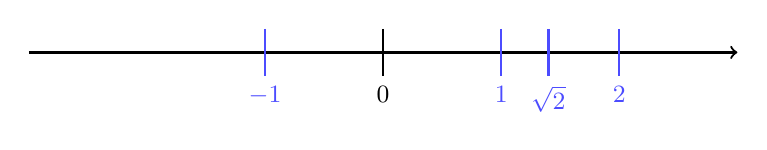
\begin{tikzpicture}[scale=1.5]
\draw[->,thick] (-3,0) -- (3,0);
\draw[below,thick] (0,.2) -- (0,-.2) node[] {\small 0};
\pause
\draw[below,thick,color=blue!70] (-1,.2) -- (-1,-.2) node[color=blue!70] {\small $-1$};
\draw[below,thick,color=blue!70] (1,.2) -- (1,-.2) node[color=blue!70] {\small $1$};
\draw[below,thick,color=blue!70] (2,.2) -- (2,-.2) node[color=blue!70] {\small $2$};
\draw[below,thick,color=blue!70] (1.4,.2) -- (1.4,-.2) node[color=blue!70] {\small $\sqrt{2}$};
\end{tikzpicture}
\end{center}
\end{itemize}}

\frame{\frametitle{Rappresentare i numeri reali}
\setstretch{1.3}
\begin{center}
\pause
consideriamo range limitato, $[a,b] \subset \mathbb{R}$
\pause
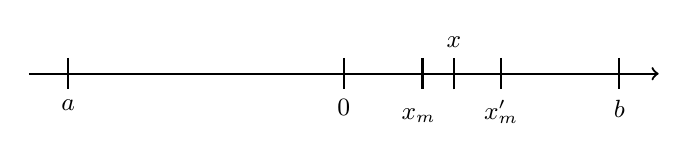
\begin{tikzpicture}[scale=1]
\draw[->,thick] (-4,0) -- (4,0);
\draw[below,thick] (-3.5,.2) -- (-3.5,-.2) node[] {\small $a$ };
\draw[below,thick] (.0,.2) -- (.0,-.2) node[] {\small $0$ };
\draw[below,thick] (3.5,.2) -- (3.5,-.2) node[] {\small $b$ };
\pause
\draw[below,thick] (1.0,.2) -- (1.0,-.2) node[] {\small $x_m\phantom{'}$ };
\draw[below,thick] (2.0,.2) -- (2.0,-.2) node[] {\small $x_m'$ };
\draw[above,thick] (1.40,-.2) -- (1.40,.2) node[] {\small $x$};
\pause
\end{tikzpicture}
\end{center}
\begin{itemize}
\item Infiniti elementi, non rappresentabili con $n$ ($<\infty$) bit
\pause
\item Rappresentazione $\mathbb{R}$ necessariamente \evi{approssimata} 
\pause
\item Usare $\mathbb{Q}$? Infiniti razionali dentro all'intervallo
\pause
\item Esatta solo per (un numero finito di) \evi{numeri macchina}
\pause
\item Num non-macchina? Approx al num macchina piu vicino
\pause
\item \evi{Errore} di rappresentazione (al massimo $\frac{x_m'-x_m}{2}$)
\end{itemize}}

\frame{\frametitle{Scegliere i numeri macchina}
\setstretch{1.3}
\begin{itemize}
\item Dati $n$ bit, rappresentare ($2^n$) numeri macchina
\pause
\item Un bit al segno, k bit per parte intera, altri a frazionaria
\pause
\item Sistema molto semplice e facile da leggere,\\ma distanza fra i numeri macchina costante
\pause
\item Es. m=8 k=4
\pause
\end{itemize}
\begin{center}
	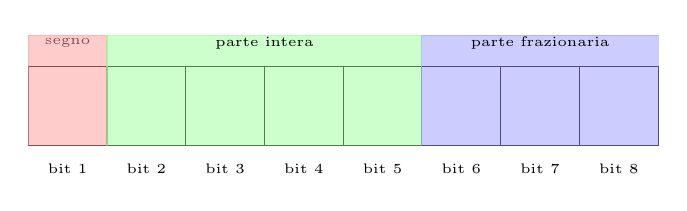
\begin{tikzpicture}
		\draw (-3,0) +(-.5,-.5) rectangle ++(.5,.5);
		\draw (-2,0) +(-.5,-.5) rectangle ++(.5,.5);
		\draw (-1,0) +(-.5,-.5) rectangle ++(.5,.5);
		\draw (0,0) +(-.5,-.5) rectangle ++(.5,.5);
		\draw (1,0) +(-.5,-.5) rectangle ++(.5,.5);
		\draw (2,0) +(-.5,-.5) rectangle ++(.5,.5);
		\draw (3,0) +(-.5,-.5) rectangle ++(.5,.5);
		\draw (4,0) +(-.5,-.5) rectangle ++(.5,.5);
		%\draw (2,0) node{$\ldots$};
		\draw (-3,-.8) node{\tiny bit $1$};
		\draw (-2,-.8) node{\tiny bit $2$};
		\draw (-1,-.8) node{\tiny bit $3$};
		\draw (0,-.8) node{\tiny bit $4$};
		\draw (1,-.8) node{\tiny bit $5$};
		\draw (2,-.8) node{\tiny bit $6$};
		\draw (3,-.8) node{\tiny bit $7$};
		\draw (4,-.8) node{\tiny bit $8$};
		\draw (-3,+.8) node{\tiny segno};
		\filldraw[color=red!40,semitransparent] (-3.5,-.50) rectangle (-2.5,.9);
		\filldraw[color=green!40,semitransparent] (-2.5,-.50) rectangle (1.5,.9);
		\filldraw[color=blue!40,semitransparent] (1.5,-.50) rectangle (4.5,.9);
		\draw (-.50,+.8) node{\tiny parte intera};
		\draw (3,+.8) node{\tiny parte frazionaria};
	\end{tikzpicture}
\end{center}
}


\frame{\frametitle{}

\begin{columns}
\begin{column}[T]{0.7\textwidth}
0 0000 000 $\to$ + $0000.000_2$ = 0\\
0 0000 001 $\to$ + $0000.001_2$ = 0.125\\
0 0000 010 $\to$ + $0000.010_2$ = 0.25\\
0 0000 011 $\to$ + $0000.011_2$ = 0.375\\
0 0000 100 $\to$ + $0000.100_2$ = 0.5\\
0 0000 101 $\to$ + $0000.101_2$ = 0.625\\
0 0000 110 $\to$ + $0000.110_2$ = 0.75\\
0 0000 111 $\to$ + $0000.111_2$ = 0.875\\
0 0001 000 $\to$ + $0001.000_2$ = 1\\

0 0001 001 $\to$ + $0000.001_2$ = 1.125\\
0 0001 010 $\to$ + $0000.010_2$ = 1.25\\
0 0001 011 $\to$ + $0000.001_2$ = 1.375\\
\quad \quad $\ldots$\\
1 1011 101$\to$ - $1011.101_2$ = -11.625\\
\end{column}
\pause
\begin{column}[T]{0.3\textwidth}
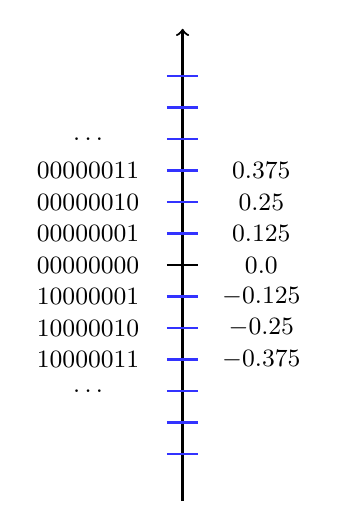
\begin{tikzpicture}[scale=1]
\draw[->,thick] (0,-3,0) -- (0,3);
\draw[thick] (-.2,0) -- (.2,0);
\draw[thick,color=blue!80] (-.2,.4) -- (.2,.4);
\draw[thick,color=blue!80] (-.2,.8) -- (.2,.8);
\draw[thick,color=blue!80] (-.2,1.2) -- (.2,1.2);
\draw[thick,color=blue!80] (-.2,1.6) -- (.2,1.6);
\draw[thick,color=blue!80] (-.2,2) -- (.2,2);
\draw[thick,color=blue!80] (-.2,2.4) -- (.2,2.4);
\draw[thick,color=blue!80] (-.2,-.4) -- (.2,-.4);
\draw[thick,color=blue!80] (-.2,-.8) -- (.2,-.8);
\draw[thick,color=blue!80] (-.2,-1.2) -- (.2,-1.2);
\draw[thick,color=blue!80] (-.2,-1.6) -- (.2,-1.6);
\draw[thick,color=blue!80] (-.2,-2) -- (.2,-2);
\draw[thick,color=blue!80] (-.2,-2.4) -- (.2,-2.4);
\draw[thick] (-1.2,-1.6) node[] {\small $\ldots$ };
\draw[thick] (-1.2,-1.2) node[] {\small $1000 0011$ }; \draw[thick] (1.,-1.2) node[] {\small $-0.375$ };
\draw[thick] (-1.2,-.8) node[] {\small $1000 0010$ }; \draw[thick] (1.,-.8) node[] {\small $-0.25$ };
\draw[thick] (-1.2,-.4) node[] {\small $1000 0001$ }; \draw[thick] (1.,-.4) node[] {\small $-0.125$ };
\draw[thick] (-1.2,0) node[] {\small $0000 0000 $ }; \draw[thick] (1.,0) node[] {\small $0.0$ };
\draw[thick](-1.2,.4) node[] {\small $0000 0001$ }; \draw[thick] (1.,.4) node[] {\small $0.125$ };
\draw[thick] (-1.2,.8) node[] {\small $0000 0010$ }; \draw[thick] (1.,.8) node[] {\small $0.25$ };
\draw[thick] (-1.2,1.2) node[] {\small $0000 0011$ }; \draw[thick] (1.,1.2) node[] {\small $0.375$ };
\draw[thick] (-1.2,1.6) node[] {\small $\ldots$ };
%\draw[below,thick] (.0,.2) -- (.0,-.2) node[] {\small $0$ };
%\draw[below,thick] (3.5,.2) -- (3.5,-.2) node[] {\small $x_{\mathrm{max}}$ };
%\draw[below,thick] (1.0,.2) -- (1.0,-.2) node[] {\small $x_m\phantom{'}$ };
%\draw[below,thick] (2.0,.2) -- (2.0,-.2) node[] {\small $x_m'$ };
%\draw[above,thick] (1.40,-.2) -- (1.40,.2) node[] {\small $x$};
\end{tikzpicture}
\pause
numeri macchina
\\
tutti \evi{equidistanti}
\\
(distanza $2^{-3}$)
\end{column}
\end{columns}
}


\frame{\frametitle{Errore assoluto e relativo}
\setstretch{1.4}
\pause
\begin{itemize}
	\item Grandezza (reale) $x$ approssimata da $x_m$
\pause
\item Errore assoluto $\epsilon_A := |x-x_m |$
\pause
\item Errore relativo $\epsilon_R := \frac{\epsilon_A}{|x|}=\left|\frac{x-x_m}{x}\right|$
\end{itemize}
\vskip 2mm
\pause
Es. 7CHF approssimati a 10CHF, $\epsilon_A=3$CHF, $\epsilon_R\simeq 43\%$
\vskip 1mm
\pause
12'007CHF approssimati a 12'010CHF, $\epsilon_A=3$CHF, $\epsilon_R\simeq 0.025\%$
\vskip 2mm
\begin{center}
\pause
per rappresentare i numeri reali \\ meglio $\epsilon_R$ indipendente dal numero che $\epsilon_A$
\end{center}
}


\frame{\frametitle{}
\setstretch{1.4}
\begin{center}
\pause
quindi anzich\'e numeri macchina equidistanti
\vskip 2mm
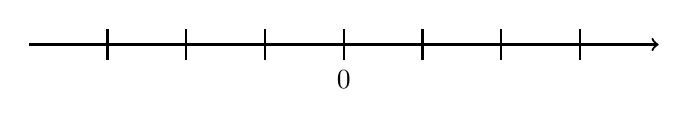
\begin{tikzpicture}[scale=1]
\draw[->,thick] (-4,0) -- (4,0);
\draw[below,thick] (.0,.2) -- (.0,-.2) node{0};
\draw[below,thick] (3,.2) -- (3,-.2) ;
\draw[below,thick] (2,.2) -- (2,-.2) ;
\draw[below,thick] (1,.2) -- (1,-.2) ;
\draw[below,thick] (-1,.2) -- (-1,-.2) ;
\draw[below,thick] (-2,.2) -- (-2,-.2) ;
\draw[below,thick] (-3,.2) -- (-3,-.2) ;
\end{tikzpicture}
\vskip 2mm
\pause
aumentare la distanza pi\`u il numero diventa grande
\vskip 1mm
(in valore assoluto)
\pause
\vskip 4mm 
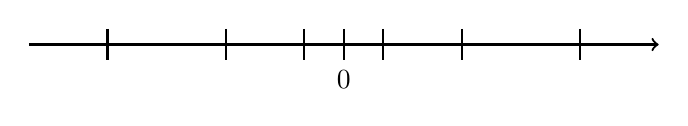
\begin{tikzpicture}[scale=1]
\draw[->,thick] (-4,0) -- (4,0);
\draw[below,thick] (.0,.2) -- (.0,-.2) node{0};
\draw[below,thick] (3,.2) -- (3,-.2) ;
\draw[below,thick] (1.5,.2) -- (1.5,-.2) ;
\draw[below,thick] (.5,.2) -- (.5,-.2) ;
\draw[below,thick] (-.5,.2) -- (-.5,-.2) ;
\draw[below,thick] (-1.5,.2) -- (-1.5,-.2) ;
\draw[below,thick] (-3,.2) -- (-3,-.2) ;
\end{tikzpicture}
\end{center}
}

\frame{\frametitle{Notazione scientifica}
\setstretch{1.2}
\begin{itemize}
\item Sistema posizionale scomodo per rappresentare numeri grandi/piccoli
\pause
\item Ex. gravitazione universale $0.000000000066725985\frac{N\cdot m^2}{kg^2},$
\pause
\item Alternativa? Notazione scientifica:
	\begin{center}
		\emph{\colorbox{red!20}{segno} per \colorbox{blue!20}{mantissa} per \colorbox{green!20}{base} elevata all'\colorbox{yellow!20}{esponente}''}
\vskip 2mm
\pause
$\colorbox{red!20}{+}$ $\colorbox{blue!20}{6.6725985} \cdot \colorbox{green!20}{10}^{\colorbox{yellow!20}{-11}}$
	\end{center}

\pause
\item Non univoco: $\colorbox{red!20}{+}$ $\colorbox{blue!20}{66.725985} \cdot \colorbox{green!20}{10}^{\colorbox{yellow!20}{-12}}$
	
\pause
	lo diventa se fisso una regola sulla mantissa
\pause
\item Stessa cosa in base due	
$\colorbox{red!20}{+}$ $\colorbox{blue!20}{1011.0011}_2 \cdot \colorbox{green!20}{2}^{\colorbox{yellow!20}{5}}$
\end{itemize}
}


\frame{\frametitle{Il formato float a 32 bit}
\setstretch{1.4}
\begin{itemize}
\pause
\item 1 bit per il segno
\item 8 bit per l'esponente
\item 32 - 1 - 8 = 23 bit per la mantissa
\pause
\end{itemize}
\begin{block}{Regole formato float (ci saranno eccezioni)}
\begin{itemize}
\pause
\item Segno: $+$ se il primo bit vale 0, $-$ altrimenti
\pause
\item Esponente: leggi gli 8 bit con Horner e togli 127 
\pause
\item Mantissa: 1.xxxx con xxx sequenza di 23 bit
\pause
\item Base: 2
\end{itemize}
\end{block}}


\frame{\frametitle{Esercizi sul formato float}
\setstretch{1.4}
\begin{enumerate}
\item Identificare a quale numero corrisponde la sequenze FA800000 e 42F91FE6 (compattata in esadecimale) sulla base delle regole del formato float
\item Identificare la sequenza di 32 bit (opportunamente compattata in esadecimale) che corrisponde al numero $x=-137.12$ secondo le regole del formato float
\item Il formato {\tt double} \`e l'analogo a 64 bit del formato float. Sapendo che il formato utilizza 11 bit per l'esponente ricostruire per analogia le regole del formato
\end{enumerate}
}

\frame{\frametitle{}
{\small FA800000 $\to 1|111\,1010\,1|000\,0000\,0000\,0000\,0000\,0000$}
\vskip 2mm
$b_1=0 \Rightarrow$ $x$ negativo
\vskip 2mm
esponente = horner($1111\,0101$)-127=118
\vskip 2mm
mantissa = 1.$0$
\vskip 2mm
$x = -2^{118}\simeq -3.3231 \cdot 10^{35}$
\begin{center}
\noindent\rule{9cm}{0.4pt}
\end{center}
{\small 42F91FE6 $\to 0|100\,0010\,1|111\,1001\,0001\,1111\,1110\,0110$}
\vskip 2mm
$b_1=0 \Rightarrow$ $x$ positivo 
\vskip 2mm
esponente =horner($1000\,0101$)-127=6
\vskip 2mm
mantissa = $1.1111001000111111110011$
\vskip 2mm
$x = 1.1111001000111111110011 \cdot 2^6 = 1111100.1000111111110011 = 124.5623016357421875$\\
}

\frame{\frametitle{}
1/2+1 = 1.5\\
1.5/2+0 = 0.75\\
0.75/2+0 = 0.375\\
0.375/2+1 = 1.1875\\
1.1875/2+1 = 1.59375\\
1.59375/2+1 = 1.796875\\
1.796875/2+1 = 1.8984375\\
1,8984375/2+1 = 1.94921875\\
1,94921875/2+1 = 1.974609375\\
1.974609375/2+1 = 1.9873046875\\
1.9873046875/2+1 = 1.99365234375\\
1.99365234375/2+0 = 0.996826171875\\
0.996826171875/2+0 = 0.4984130859375\\
0.4984130859375/2+0 = 0.24920654296875\\
0.24920654296875/2+1 = 1.124603271484375\\
1.124603271484375/2 = 0.5623016357421875\\
}

\frame{\frametitle{}
Sequenza 32 bit associata a $-137.12_{10}$ secondo float 
\begin{columns}
\begin{column}[T]{0.4\textwidth}
	$137_{10}$ in base 2
\vskip 2mm
$137 \mod 2 = 1$\\ 
$68 \mod 2 = 0$\\ 
$34 \mod 2 = 0$\\ 
$17 \mod 2 = 1$\\ 
$8 \mod 2 = 0$\\ 
$4 \mod 2 = 0$\\ 
$2 \mod 2 = 0$\\ 
$1 \mod 2 = 1$\\ 
$0/$
\vskip 2mm
Sintesi: $137_{10}=10001001_2$\\
\vskip 1mm 
Verifica: $137=2^{7}+2^3+1$
\end{column}
\begin{column}[T]{0.6\textwidth}
\small
	$0.12_{10}=0.\overline{00011110101110000100}_2$ 
\tiny
\vskip 4mm
$int(0.12 \cdot 2) = 0$\\
$int(0.24\cdot 2) = 0$\\
$int(0.48\cdot 2) = 0$\\
$int(0.96\cdot 2) = 1$\\
$int(0.92\cdot 2) = 1$\\
$int(0.84\cdot 2) = 1$\\
$int(0.68\cdot 2) = 1$\\
$int(0.36\cdot 2) = 0$\\
$int(0.72\cdot 2) = 1$\\
$int(0.44\cdot 2) = 0$\\
$int(0.88\cdot 2) = 1$\\
$int(0.76\cdot 2) = 1$\\
$int(0.52\cdot 2) = 1$\\
$int(0.04\cdot 2) = 0$\\
$int(0.08\cdot 2) = 0$\\
$int(0.16\cdot 2) = 0$\\
$int(0.32\cdot 2) = 0$\\
$int(0.64\cdot 2) = 1$\\
$int(0.28\cdot 2) = 0$\\
$int(0.56\cdot 2) = 0$\\
$int(0.12\cdot 2) = 0$\\periodico!\\
\end{column}
\end{columns}
}

\frame{\frametitle{}
$-137.12=-10001001.\overline{00011110101110000100}_2$ 
\vskip 2mm
Notazione scientifica
$-10001001.\overline{00011110101110000100}_2 \cdot 2^0$ 
\vskip 2mm
Mantissa normalizzata
$-1.0001001\overline{00011110101110000100}_2 \cdot 2^7$ 
\vskip 2mm
Quasi-formato float
$-1.0001001\overline{00011110101110000100}_2 \cdot 2^{134-127}$ 
\vskip 2mm
Rappresento 134 a 8 bit
\small
\vskip 2mm
$134 \mod 2=0$\\
$67 \mod 2=1$\\
$33\mod 2=1$\\
$16 \mod 2=0$\\
$8\mod 2=0$\\
$4 \mod 2=0$\\
$2\mod 2=0$\\
$1 \mod 2=1$\\
\vskip 2mm
$134_{10} = 10000110_2$\\
}
\frame{
\frametitle{}
$-137.12 = -1.0001001\overline{00011110101110000100}_2 \cdot 2^{\mathrm{horner}(10000110)-127}$ 
\vskip 2mm
23 bit per la mantissa
\vskip 2mm
$-1.\colorbox{yellow}{00010010001111010111000}0100 \ldots  \cdot 2^{\mathrm{horner}(10000110)-127}$ 


\begin{center}
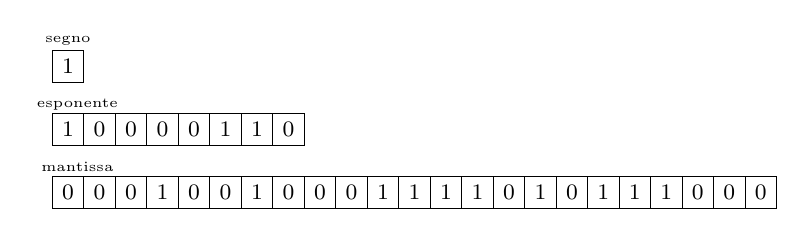
\begin{tikzpicture}[scale=.4]
\draw (0,+.8) node{\tiny segno};
\draw (0,0) +(-.5,-.5) rectangle ++(.5,.5); 
\draw (0,0) node{\footnotesize $1$}; 
\draw (.3,-1.2) node{\tiny esponente};
\draw (0,-2) +(-.5,-.5) rectangle ++(.5,.5); 
\draw (1,-2) +(-.5,-.5) rectangle ++(.5,.5); 
\draw (2,-2) +(-.5,-.5) rectangle ++(.5,.5); 
\draw (3,-2) +(-.5,-.5) rectangle ++(.5,.5); 
\draw (4,-2) +(-.5,-.5) rectangle ++(.5,.5); 
\draw (5,-2) +(-.5,-.5) rectangle ++(.5,.5); 
\draw (6,-2) +(-.5,-.5) rectangle ++(.5,.5); 
\draw (7,-2) +(-.5,-.5) rectangle ++(.5,.5); 
\draw (0,-2) node{\footnotesize $1$}; 
\draw (1,-2) node{\footnotesize $0$}; 
\draw (2,-2) node{\footnotesize $0$};
\draw (3,-2) node{\footnotesize $0$};
\draw (4,-2) node{\footnotesize $0$};
\draw (5,-2) node{\footnotesize $1$};
\draw (6,-2) node{\footnotesize $1$};
\draw (7,-2) node{\footnotesize $0$};
\draw (.3,-3.2) node{\tiny mantissa};
\draw (0,-4) +(-.5,-.5) rectangle ++(.5,.5); 
\draw (1,-4) +(-.5,-.5) rectangle ++(.5,.5); 
\draw (2,-4) +(-.5,-.5) rectangle ++(.5,.5); 
\draw (3,-4) +(-.5,-.5) rectangle ++(.5,.5); 
\draw (4,-4) +(-.5,-.5) rectangle ++(.5,.5); 
\draw (5,-4) +(-.5,-.5) rectangle ++(.5,.5); 
\draw (6,-4) +(-.5,-.5) rectangle ++(.5,.5); 
\draw (7,-4) +(-.5,-.5) rectangle ++(.5,.5); 
\draw (8,-4) +(-.5,-.5) rectangle ++(.5,.5); 
\draw (9,-4) +(-.5,-.5) rectangle ++(.5,.5); 
\draw (10,-4) +(-.5,-.5) rectangle ++(.5,.5); 
\draw (11,-4) +(-.5,-.5) rectangle ++(.5,.5); 
\draw (12,-4) +(-.5,-.5) rectangle ++(.5,.5); 
\draw (13,-4) +(-.5,-.5) rectangle ++(.5,.5); 
\draw (14,-4) +(-.5,-.5) rectangle ++(.5,.5); 
\draw (15,-4) +(-.5,-.5) rectangle ++(.5,.5); 
\draw (16,-4) +(-.5,-.5) rectangle ++(.5,.5); 
\draw (17,-4) +(-.5,-.5) rectangle ++(.5,.5); 
\draw (18,-4) +(-.5,-.5) rectangle ++(.5,.5); 
\draw (19,-4) +(-.5,-.5) rectangle ++(.5,.5); 
\draw (20,-4) +(-.5,-.5) rectangle ++(.5,.5); 
\draw (21,-4) +(-.5,-.5) rectangle ++(.5,.5); 
\draw (22,-4) +(-.5,-.5) rectangle ++(.5,.5); 
\draw (0,-4) node{\footnotesize $0$}; 
\draw (1,-4) node{\footnotesize $0$}; 
\draw (2,-4) node{\footnotesize $0$}; 
\draw (3,-4) node{\footnotesize $1$}; 
\draw (4,-4) node{\footnotesize $0$}; 
\draw (5,-4) node{\footnotesize $0$}; 
\draw (6,-4) node{\footnotesize $1$}; 
\draw (7,-4) node{\footnotesize $0$}; 
\draw (8,-4) node{\footnotesize $0$}; 
\draw (9,-4) node{\footnotesize $0$}; 
\draw (10,-4) node{\footnotesize $1$}; 
\draw (11,-4) node{\footnotesize $1$}; 
\draw (12,-4) node{\footnotesize $1$}; 
\draw (13,-4) node{\footnotesize $1$}; 
\draw (14,-4) node{\footnotesize $0$}; 
\draw (15,-4) node{\footnotesize $1$}; 
\draw (16,-4) node{\footnotesize $0$}; 
\draw (17,-4) node{\footnotesize $1$}; 
\draw (18,-4) node{\footnotesize $1$}; 
\draw (19,-4) node{\footnotesize $1$}; 
\draw (20,-4) node{\footnotesize $0$}; 
\draw (21,-4) node{\footnotesize $0$}; 
\draw (22,-4) node{\footnotesize $0$}; 
\end{tikzpicture}
\end{center}
\vskip 2mm
Sintesi $1|10000110|00010010001111010111000$ 
\vskip 2mm
Zip esadecimale
\vskip 2mm
\small
1100 0011 0000 1001 0001 1110 1011 1000 $\to$ C 3 0 9 1 E B 8 
}
\frame{\frametitle{}
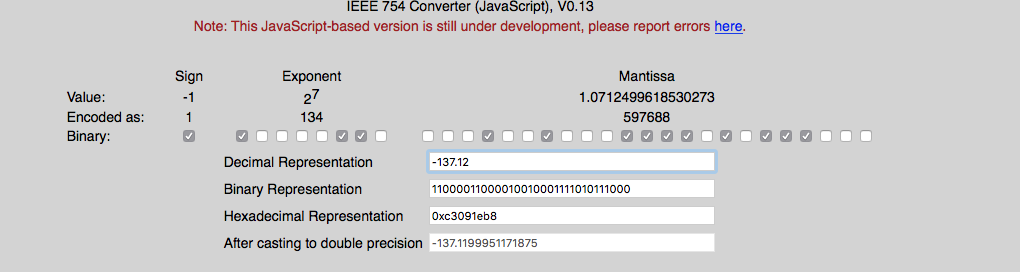
\includegraphics[width=11cm]{conversion}
}

\frame{\frametitle{From 32 to 64}
\begin{itemize} 
\item {\Large Float (32 bit)}
\end{itemize}
\begin{center}	
	$x = {\color{red!40}{\mathrm{sgn}(b_1)}} \cdot 1.{\color{blue!40}{[b_{10},\ldots,b_{32}]}} \cdot 2^{{\color{black!60!green}{\mathrm{HORNER}(b_2,\ldots,b_9)}}-127}$
\end{center}	
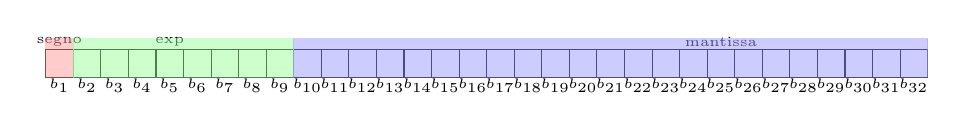
\begin{tikzpicture}[scale=.35]
\foreach \i in {1,...,32} {\draw (\i,0) +(-.5,-.5) rectangle ++(.5,.5); 
\draw (\i,-.8) node[font=\fontsize{3}{3.5}\selectfont]{$b_{\i}$};}
\draw (1,.8) node[font=\fontsize{3}{3.5}\selectfont]{segno};
\draw (5,.8) node[font=\fontsize{3}{3.5}\selectfont]{exp};
\draw (25,.8) node[font=\fontsize{3}{3.5}\selectfont]{mantissa};
\filldraw[color=red!40,semitransparent] (.5,-.50) rectangle (1.5,.9);
\filldraw[color=green!40,semitransparent] (1.5,-.50) rectangle (9.5,.9);
\filldraw[color=blue!40,semitransparent] (9.5,-.50) rectangle (32.5,.9);
\end{tikzpicture}
\vskip 2mm
\begin{itemize} 
	\item {\Large Double (64 bit)}
\end{itemize}
\begin{center}	
$x = {\color{red!40}{\mathrm{sgn}(b_1)}} \cdot 1.{\color{blue!40}{[b_{13},\ldots,b_{64}]}} \cdot 2^{{\color{black!60!green}{\mathrm{HORNER}(b_2,b_{12})}}-1023}$
\end{center}	
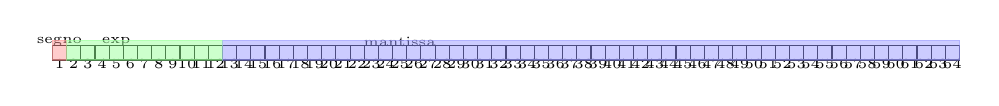
\begin{tikzpicture}[scale=.18]
\foreach \i in {1,...,64} {\draw (\i,0) +(-.5,-.5) rectangle ++(.5,.5); 
\draw (\i,-.8) node[font=\fontsize{3}{3.5}\selectfont]{\i};}
\draw (1,.8) node[font=\fontsize{3}{3.5}\selectfont]{segno};
\draw (5,.8) node[font=\fontsize{3}{3.5}\selectfont]{exp};
\draw (25,.8) node[font=\fontsize{3}{3.5}\selectfont]{mantissa};
\filldraw[color=red!40,semitransparent] (.5,-.50) rectangle (1.5,.9);
\filldraw[color=green!40,semitransparent] (1.5,-.50) rectangle (12.5,.9);
\filldraw[color=blue!40,semitransparent] (12.5,-.50) rectangle (64.5,.9);
\end{tikzpicture}
\vskip 2mm
$\mathrm{sgn}(b) = (-1)^b$, $127 = 2^{\mathbf{8}-1}-1$, $1023 = 2^{\mathbf{11}-1}-1$}

\end{document}
